\begingroup
\definecolor{coverink}{HTML}{17293C}
\definecolor{coverborder}{HTML}{C3CFD8}
\definecolor{coverpanel}{HTML}{F3F6F8}
\definecolor{coverseq}{HTML}{486E91}
\definecolor{coverjoint}{HTML}{196D60}
\definecolor{coverunknown}{HTML}{D9BE9C}
\resizebox{\linewidth}{!}{%
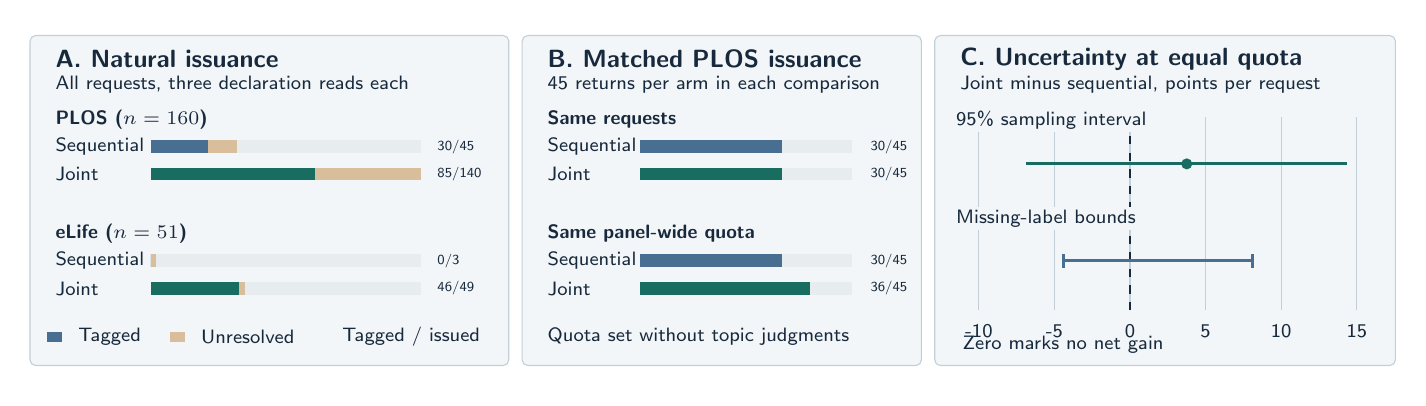
\begin{tikzpicture}[x=1cm,y=1cm,color=coverink,font=\sffamily\scriptsize,
  heading/.style={anchor=west,font=\sffamily\small\bfseries},
  panel/.style={rounded corners=2pt,draw=coverborder,fill=coverpanel}]
  \path[use as bounding box] (0,0) rectangle (17.4,4.45);
  \draw[panel] (.03,.16) rectangle (6.11,4.35);
  \draw[panel] (6.28,.16) rectangle (11.35,4.35);
  \draw[panel] (11.52,.16) rectangle (17.37,4.35);

  \node[heading] at (.23,4.05) {A. Natural issuance};
  \node[heading] at (6.48,4.05) {B. Matched PLOS issuance};
  \node[heading] at (11.72,4.05) {C. Uncertainty at equal quota};
  \node[anchor=west] at (.23,3.72) {All requests, three declaration reads each};
  \node[anchor=west] at (6.48,3.72) {45 returns per arm in each comparison};
  \node[anchor=west] at (11.72,3.72) {Joint minus sequential, points per request};

  \node[anchor=west,font=\sffamily\bfseries\scriptsize] at (.23,3.28) {PLOS ($n=160$)};
  \node[anchor=west,font=\sffamily\bfseries\scriptsize] at (.23,1.84) {eLife ($n=51$)};
  \foreach \label/\y/\known/\total/\tone in {
    Sequential/2.94/30/45/coverseq,Joint/2.59/85/140/coverjoint,
    Sequential/1.49/0/3/coverseq,Joint/1.14/46/49/coverjoint} {
    \node[anchor=west] at (.23,\y) {\label};
    \fill[coverborder!40] (1.56,{\y-.08}) rectangle (4.99,{\y+.08});
    \fill[\tone] (1.56,{\y-.08}) rectangle ({1.56+.0245*\known},{\y+.08});
    \fill[coverunknown] ({1.56+.0245*\known},{\y-.08}) rectangle ({1.56+.0245*\total},{\y+.08});
    \node[anchor=west,font=\sffamily\tiny] at (5.08,\y) {\known/\total};
  }
  \fill[coverseq] (.25,.46) rectangle (.44,.58);
  \node[anchor=west] at (.52,.52) {Tagged};
  \fill[coverunknown] (1.81,.46) rectangle (2.00,.58);
  \node[anchor=west] at (2.08,.52) {Unresolved};
  \node[anchor=east] at (5.87,.52) {Tagged / issued};

  \node[anchor=west,font=\sffamily\bfseries\scriptsize] at (6.48,3.28) {Same requests};
  \node[anchor=west,font=\sffamily\bfseries\scriptsize] at (6.48,1.84) {Same panel-wide quota};
  \foreach \label/\y/\known/\tone in {
    Sequential/2.94/30/coverseq,Joint/2.59/30/coverjoint,
    Sequential/1.49/30/coverseq,Joint/1.14/36/coverjoint} {
    \node[anchor=west] at (6.48,\y) {\label};
    \fill[coverborder!40] (7.78,{\y-.08}) rectangle (10.47,{\y+.08});
    \fill[\tone] (7.78,{\y-.08}) rectangle ({7.78+.0598*\known},{\y+.08});
    \node[anchor=west,font=\sffamily\tiny] at (10.58,\y) {\known/45};
  }
  \node[anchor=west] at (6.48,.52) {Quota set without topic judgments};

  \foreach \value in {-10,-5,0,5,10,15} {
    \draw[coverborder] ({12.08+.192*(\value+10)},.86) -- ({12.08+.192*(\value+10)},3.31);
    \node[anchor=north] at ({12.08+.192*(\value+10)},.80) {\value};
  }
  \draw[coverink,dashed] ({12.08+.192*10},.86) -- ({12.08+.192*10},3.31);
  \node[anchor=west,fill=coverpanel,inner sep=1pt] at (11.75,3.27) {95\% sampling interval};
  \node[anchor=west,fill=coverpanel,inner sep=1pt] at (11.75,2.03) {Missing-label bounds};
  \draw[coverjoint,line width=1.1pt] ({12.08+.192*3.10},2.72) -- ({12.08+.192*24.37},2.72);
  \fill[coverjoint] ({12.08+.192*13.75},2.72) circle (2pt);
  \draw[coverseq,line width=1.1pt] ({12.08+.192*5.625},1.49) -- ({12.08+.192*18.125},1.49);
  \foreach \value in {5.625,18.125}
    \draw[coverseq,line width=1.1pt] ({12.08+.192*\value},1.40) -- ({12.08+.192*\value},1.58);
  \node[anchor=west] at (11.75,.42) {Zero marks no net gain};
\end{tikzpicture}%
}
\endgroup
